\documentclass[12pt]{article}
\usepackage[margin = 1.5in]{geometry}
\setlength{\parindent}{0in}
\usepackage{amsfonts, amssymb, amsthm, mathtools, tikz, qtree, float}
\usepackage[lined]{algorithm2e}
\usepackage[T1]{fontenc}
\usepackage{ae, aecompl, color}
\usepackage[pdftex, pdfauthor={Charles Shen}, pdftitle={CS 251: Computer Organization and Design}, pdfsubject={Lecture notes from CS 251: Computer Organization and Design at the University of Waterloo}, pdfkeywords={CS 251, course notes, notes, Waterloo, University of Waterloo}, pdfproducer={LaTeX}, pdfcreator={pdflatex}]{hyperref}
\usepackage{cleveref}
\usepackage{wrapfig}

\DeclarePairedDelimiter{\set}{\lbrace}{\rbrace}

\definecolor{darkish-blue}{RGB}{25,103,185}

\hypersetup{
  colorlinks,
  citecolor=darkish-blue,
  filecolor=darkish-blue,
  linkcolor=darkish-blue,
  urlcolor=darkish-blue
}

\theoremstyle{definition}
\newtheorem*{defn}{Definition}
\newtheorem*{theorem}{Theorem}
\newtheorem*{corollary}{Corollary}
\newtheorem{ex}{Example}[section]

\crefname{ex}{Example}{Example}

\setlength{\marginparwidth}{1.5in}
\newcommand{\lecture}[1]{
  \marginpar{{
    \footnotesize $\leftarrow$ \underline{#1}}
  }
}

\newcommand{\includePicture}[3]{
  \begin{figure}[!h]
  \centering
  \scalebox{#1}{\includegraphics{#2}}
  \caption{#3}
  \end{figure}
}

\allowdisplaybreaks

\makeatletter
\def\blfootnote{\gdef\@thefnmark{}\@footnotetext}
\makeatother

%%%%%%%%%%%%%%%%%%%%%
%% D O C U M E N T %%
%%%%%%%%%%%%%%%%%%%%%

\begin{document}
  \let\ref\Cref

  \title{\bf{CS 251: Computer Organization and Design}}
  \date{Spring 2016, University of Waterloo \\ \center Notes written from Safaa Bedawi's lectures.}
  \author{Charles Shen}

  \blfootnote{Feel free to email feedback to me at
  \href{mailto:echen902@gmail.com}{echen902@gmail.com}.}

  \maketitle
  \newpage
  \tableofcontents
  \newpage

  \section{From Zero To One, Abstractions}
  \includePicture{0.6}{pictures/abstractionLevel.png}{Levels of abstraction for electronic computing system}

  \subsection{The Three -Y's}
  \begin{itemize}
    \item [\textbf{Hierarchy}] involves dividing a system into modules, then further subdividing each of these modules until the pieces are easy to understand
    \item [\textbf{Modularity}] states that the modules have well-defined functions and interfaces, so that they connect together easily without unanticipated side effects
    \item [\textbf{Regularity}] seeks uniformity among the modules. Common modules are reused many times, reducing the number of distinct modules that must be designed
  \end{itemize}

  \subsection{Hexadecimal Number System}
  \begin{tabular} {c | c | c}
  Hexadecimal Digit & Decimal Digit & Binary Equivalent \\ \hline
  0 & 0 & 0000 \\ \hline
  1 & 1 & 0001 \\ \hline
  2 & 2 & 0010 \\ \hline
  3 & 3 & 0011 \\ \hline
  4 & 4 & 0100 \\ \hline
  5 & 5 & 0101 \\ \hline
  6 & 6 & 0110 \\ \hline
  7 & 7 & 0111 \\ \hline
  8 & 8 & 1000 \\ \hline
  9 & 9 & 1001 \\ \hline
  A & 10 & 1010 \\ \hline
  B & 11 & 1011 \\ \hline
  C & 12 & 1100 \\ \hline
  D & 13 & 1101 \\ \hline
  E & 14 & 1110 \\ \hline
  F & 15 & 1111 \\
  \end{tabular}

  \subsection{Bytes, Nibbles, and All That Jazz}
  A group of eight bits is called a byte. Represents $256 = 2^{8}$ possibilities. \\
  A group of four bits is called a nibble. Represents $16 = 2^{4}$ possibilities. \\
  A microprocessor is a processor built on a single chip. \\
  Microprocessors handle data in chunks called words. The size of a word depends on the architecture of the microprocessor. \\
  Within a group of bits, the bit in the 1's column is called the least significant bit (lsb), and the bit at the other end is called the most significant bit (msb). \\
  Within a word, the bytes are identified as least significant byte (LSB) through most significant byte (MSB). \\

  \blfootnote{When adding operands with different signs, overflow cannot occur because the sum must be no larger than one of the operands.}
  \newpage

  \subsection{Logic Gates}
  A circuit element that performs a basic logic function \\ \\
  \textbf{Single Input} \\
  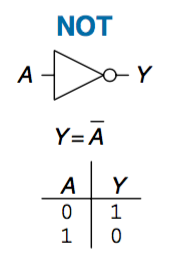
\includegraphics[scale=0.9]{pictures/notGate.png}
  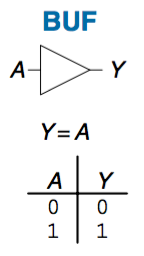
\includegraphics[scale=0.9]{pictures/bufGate.png} \\
  \textbf{Double Output} \\
  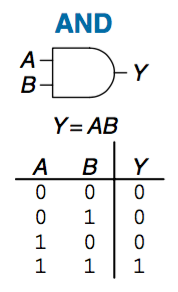
\includegraphics[scale=0.9]{pictures/andGate.png}
  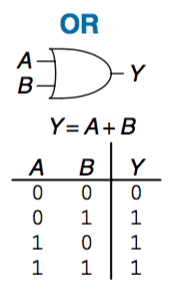
\includegraphics[scale=0.9]{pictures/orGate.png}
  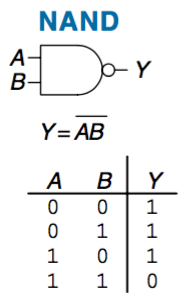
\includegraphics[scale=0.9]{pictures/nandGate.png}
  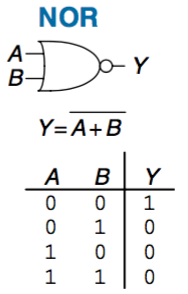
\includegraphics[scale=0.9]{pictures/norGate.png}
  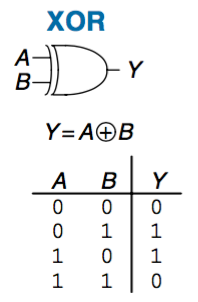
\includegraphics[scale=0.9]{pictures/xorGate.png}

  \subsection{Beneath the Digital Abstraction}
  A digital system uses discrete-valued variables. \\
  Variables are represented by continuous physical quantities such as the voltage on a wire, the position of a gear, or the level of fluid in a cylinder. \\ \\
  For example: \\
  Consider representing a binary signal A with a voltage on a wire. \\
  Let 0 volts (V) indicate A = 0 and 5V indicate A = 1. \\
  Any real system must tolerate some noise, so 4.97V probably ought to be interpreted as A = 1 as well. \\
  But what about 4.3V? Or 2.8V? Or 2.5000000V?

  \subsubsection{Supply Voltage}
  Suppose the lowest voltage in the system is 0V, also called ground or GND \\
  The highest voltage in the system comes from the power supply and is usually called $V_{DD}$

  \subsubsection{Logic Levels}
  Mapping of a continuous variable onto a discrete binary variable is done by defining logic levels.
  First gate is called the driver and the second gate is called the receiver.
  Output of the driver is connected to the input of the receiver. \\
  The driver produces a LOW (0) output in the range of 0 to $V_{OL}$ or a HIGH (1) output in the range of $V_{OH}$ to $V_{DD}$

  \subsubsection{Noise Margins}
  If the output of the driver is to be correctly interpreted at the input of the receiver, we must choose $V_{OL} < V_{IL}$ and $V_{OH} > V_{IH}$ \\
  Even if the output of the driver is contaminated by some noise, the input of the receiver will still detect the correct logic level.
  Noise margin is the amount of noise that could be added to a worst-case output such that the signal can still be interpreted as a valid input.

  \subsubsection{DC Transfer Characteristics}
  The DC transfer characteristics of a gate describe the output voltage as a function of the input voltage when the input is changed slowly enough that the output can keep up. \\
  Called transfer characteristics because they describe the relationship between input and output voltages.

  \section{CMOS Transistors}
  Transistors are electrically controlled switches that turn ON or OFF when a voltage or current is applied to a control terminal. \\
  Two main types of transistors are bipolar transistors and metal-oxide-semiconductor field effect transistors (MOSFETs or MOS transistors).

  \subsection{Semiconductors}
  MOS transistors are built from silicon. \\
  Silicon has four electrons in its valence shell and forms bonds with four adjacent atoms, resulting in a crystalline lattice. \\
  By itself, silicon is a poor conductor due to all the electrons are tied up in covalent bonds. \\
  Becomes a better conductor when small amounts of impurities, called dopant atoms, are added. \\
  The conductivity of silicon changes over many orders and of magnitude depending on the concentration of dopants, silicon is called a semiconductor. \\
  \textbf{Add Arsenic} \\
  If arsenic (As), a group V dopant, is added, the dopant atoms have an extra electron that is not involved in the bonds. \\
  Electron can easily move about the lattice, leaving an ionized dopant atom (As+) behind. \\
  Electron carries a negative charge, so arsenic is an n-type dopant. \\
  \textbf{Add Boron} \\
  If boron (B), a group III dopant, is added, the dopant atoms are missing an electron. \\
  The missing electron is called a hole. \\
  An electron from a neighboring silicon atom may move over to fill the missing bond, forming an ionized dopant atom (B-) and leaving a hole at the neighboring silicon atom. \\
  The hole can migrate around the lattice. \\
  Hole is a lack of negative charge, so it acts like a positively charged particle. \\
  So boron is a p-type dopant.

  \subsection{Diodes}
  \begin{wrapfigure}{r}{0.25\textwidth}
    \centering
    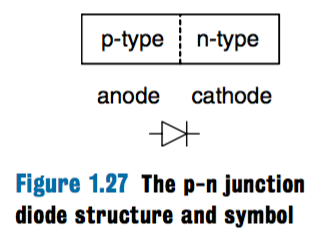
\includegraphics[width=0.25\textwidth]{pictures/diode.png}
  \end{wrapfigure}
  Junction between p-type and n-type silicon is called a diode.
  The p-type region is called the anode and the n-type region is called the cathode. \\
  When the voltage on the anode rises above the voltage on the cathode, the diode is forward biased, and current flows through the diode from the anode to the cathode. \\
  When the anode voltage is lower than the voltage on the cathode, the diode is reverse biased, and no current flows. \\
  The diode symbol intuitively shows that current only flows in one direction.

  \subsection{Capacitors}
  A \emph{capacitor} consists of two conductors separated by an insulator. \\
  When a voltage $V$ is applied to one of the conductors, the conductor accumulates electric \emph{charge} $Q$ and the other conductor accumulates the opposite charge $-Q$. \\
  The \emph{capacitance} C of the capacitor is the ratio of charge to voltage: $C = \frac{Q}{V}$.
  The capacitance is proportional to the size of the conductors and inversely proportional the distance between them. \\
  Capacitance is important because charing or discharging a conductor takes time and energy. More capacitance means that a circuit will be slower and require more energy to operate.

  \subsection{nMOS and pMOS Transistors}
  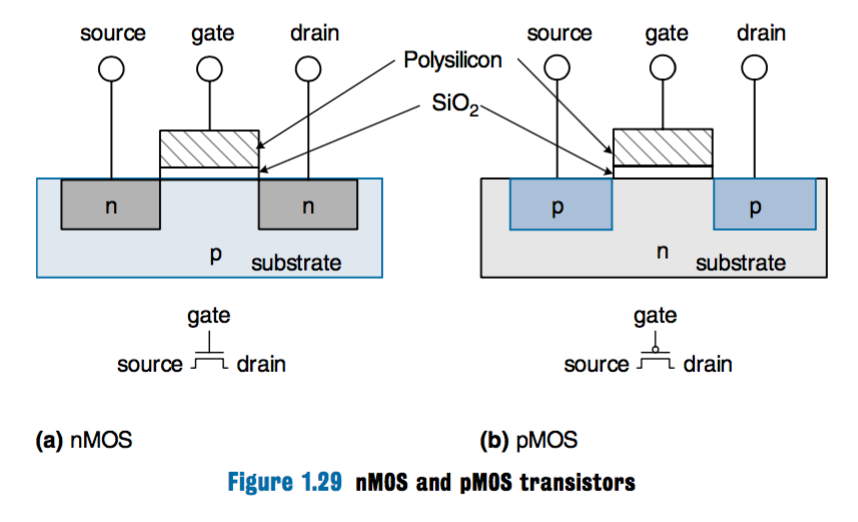
\includegraphics{pictures/nMOSpMOS.png} \\
  A MOSFET is a sandwich of several layers of conducting and insulating materials. \\
  There are two flavors of MOSFETs: nMOS and pMOS. \\
  The n-type transistors, called \emph{nMOS}, have regions of n-type dopants adjacent tot he gate called the \emph{source} and the \emph{drain} and are built on a p-type semiconductor substrate. \\
  The \emph{pMOS} transistors are just the opposite, consisting of p-type source and drain regions in an n-type \emph{substrate}. \\
  A MOSFET behaves as a voltage-controlled switch in which the gate voltage creates an electric field that turns ON or OFF a connection between the source and drain. \\
  nMOS transistors pass 0's well but passes 1's poorly.
  Similarly, pMOS transistors pass 1's well but 0's poorly. \\
  nMOS transistors need a p-type substrate, and pMOS transistors need an n-type substrate.
  To build both flavors of transistors on the same chip, manufacturing processes typically start with a p-type wafer, then implant n-type region called wells where the pMOS transistors should go.
  These processes that provide both flavors of transistors are called Complementary MOS or CMOS.
  \begin{wrapfigure}{r}{0.5\textwidth}
    \centering
    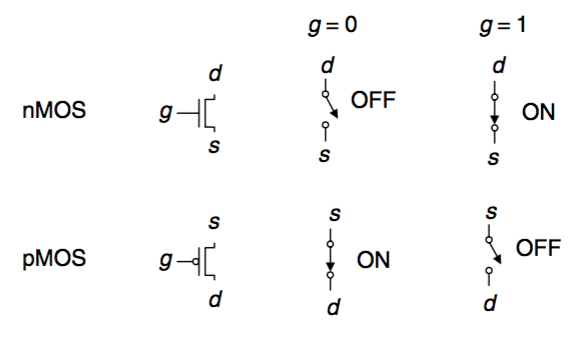
\includegraphics[width=0.5\textwidth]{pictures/nMOSpMOSGate.png}
  \end{wrapfigure}
  CMOS processes are used to build the vast majority of all transistors fabricated today. \\
  CMOS processes provide two types of electrically controlled switches.
  nMOS transistors are OFF when the gate is 0 and ON when the gate is 1.
  pMOS transistors are just the opposite: ON when the gate is 0 and OFF when the gate is 1.

  \subsection{Transmission Gates}
  \begin{wrapfigure}{r}{0.15\textwidth}
    \centering
    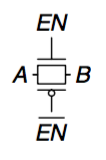
\includegraphics[width=0.15\textwidth]{pictures/transmissionGate.png}
  \end{wrapfigure}
  At times, designers find it convenient to use an ideal switch that can pass both 0 and 1 well. \\
  nMOS transistors are good at passing 0 and pMOS transistors are good at passing 1, so the parallel combination of the two passes both values well. \\
  Image to the right shows such a circuit, called \emph{transmission gate \emph{or} pass gate}. \\
  The two sides of the switch are called \emph{A \emph{and} B} because a switch is bidirectional and has no preferred input or output side.
  The control signals are called \emph{enables}, $EN$ and $\overline{EN}$. \\
  When $EN = 0$ and $\overline{EN} = 1$, both transistors are OFF.
  Hence, the transmission gate is OFF or disabled, so A and B are not connected. \\
  When $EN = 1$ and $\overline{EN} = 0$, the transmission is ON or enabled, and any logic value can flow between A and B.

  \subsection{Pseudo-nMOS Logic}
  An \emph{N}-input CMOS NOR gate uses \emph{N} nMOS transistors in parallel and \emph{N} pMOS transistors in series.
  Transistors in series are slower than transistors in parallel, just as resistors in series have more resistance than resistors in parallel. \\
  Moreover, pMOS transistors are slower than nMOS transistors because holes cannot move around the silicon lattice as fast as electrons.
  Therefore parallel nMOS transistors are fast and the series pMOS transistors are slow, especially when many are in series. \\

  Pseudo-nMOS logic replaces the slow stack of pMOS transistors with a single weak pMOS transistor that is always ON.
  This pMOS transistors is often called a \emph{weak pull-up}.
  The physical dimensions of the pMOS transistor are selected so that the pMOS transistor will pull the output, $Y$, HIGH weakly---that is, only if none of the nMOS transistors are ON.
  But if any nMOS transistor is ON, it overpowers the weak pull-up and pulls Y down close enough to GND to produce a logic 0. \\

  The advantage of pseudo-nMOS logic is that it can be used to build fast NOR gates with many inputs. \\
  The disadvantage is that a short circuit exists between $V_{DD}$ and GND when the output is LOW; the weak pMOS and nMOS transistors are both ON.
  The short circuit draws continuous power, so pseudo-nMOS logic must be used sparingly.

  \section{Summary So Far}
  \emph{There are 10 kinds of people in this world: those who can count in
binary and those who can't.} \\
  The real world is analog, though digital designers discipline themselves to use a discrete subset of possible signals.
  In particular, binary variables have just two states: 0 and 1, also called FALSE and TRUE or LOW and HIGH. \\

  Logic gates compute a binary output from one or more binary inputs.
  Some of the common logic gates are:
  \begin{itemize}
    \item[\textbf{NOT}:] TRUE when all input is FALSE
    \item[\textbf{AND}:] TRUE when all input are TRUE
    \item[\textbf{OR}:]  TRUE when any inputs are TRUE
    \item[\textbf{XOR}:] TRUE when an odd number of inputs are TRUE
  \end{itemize}

  Logic gates are commonly built from CMOS transistors, which behave as electrically controlled switches. \\
  nMOS transistors turn ON when the gate is 1. \\
  pMOS transistors turn ON when the gate is 0.

  \section{Introduction to Combinational Logic Design}
  In digital electronics, a \emph{circuit} is a network that processes discrete-valued variables. \\
  A circuit can be viewed as a black box, with
  \begin{itemize}
    \item one or more discrete-valued \emph{input terminals}
    \item one or more discrete-valued \emph{output terminals}
    \item a \emph{functional specification} describing the relationship between inputs and outputs
    \item a \emph{timing specification} describing the delay between inputs changing and output responding
  \end{itemize}
  Peeing inside the black box, circuits are composed of nodes and elements. \\
  An \emph{element} is itself a circuit with inputs, outputs, and a specification. \\
  A \emph{node} is a wire, whose voltage coveys a discrete-valued variable.
  Nodes are classified as \emph{input, output, \emph{or} internal}. \\
  Input receive values from the external world. \\
  Output deliver values to the external world. \\
  Wires that are not inputs or outputs are called internal nodes. \\

  Digital circuits are classified as \emph{combinational \emph{or} sequential}. \\
  A combinational circuit's outputs depend only on the current values of the inputs; in other words, it combines the current input values to compute the output.
  For example, a logic gate is a combinational circuit. \\
  A sequential circuit's outputs depend on both current and previous values of the inputs; in other words, it depends on the input sequence. \\
  A combinational circuit is \emph{memoryless}, but a sequential circuit has \emph{memory}. \\

  The functional specification of a combination circuit expresses the output values in terms of the current input values. \\
  The timing specification of a combinational circuit consists of lower and upper bounds on the delay from input to put. \\

  To simply drawings, a single line with a slash through it and a number next to it is often used to indicate a \emph{bus}, a bundle of of multiple signals.
\\
  \begin{wrapfigure}{l}{0.25\textwidth}
    \centering
    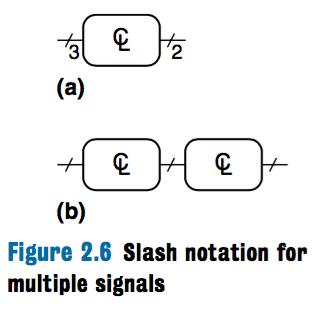
\includegraphics[width=0.25\textwidth]{pictures/busExample.png}
  \end{wrapfigure}
  In Figure 2.6(a), it represents a block of combination logic with three inputs and output outputs. \\
  If the number of bits is unimportant or obvious from the context, the slash may be shown without a number. \\
  Figure 2.6(b) indicates two blocks of combinational logic with an arbitrary number of outputs from one block serving as inputs to the second block. \\

  The rules of \emph{combinational composition} tell us how we can build a large combinational circuit from smaller combinational circuit elements. \\
  A circuit is combinational if it consists of interconnected circuit elements such that:
  \begin{itemize}
    \item Every circuit element is itself combinational
    \item Every node of the circuit is either designated as an input to the circuit or connects to exactly one output terminal of a circuit element
    \item The circuit contains no cyclic paths: every path through the circuit visits each circuit node at most once
  \end{itemize}

  Examples: \\
  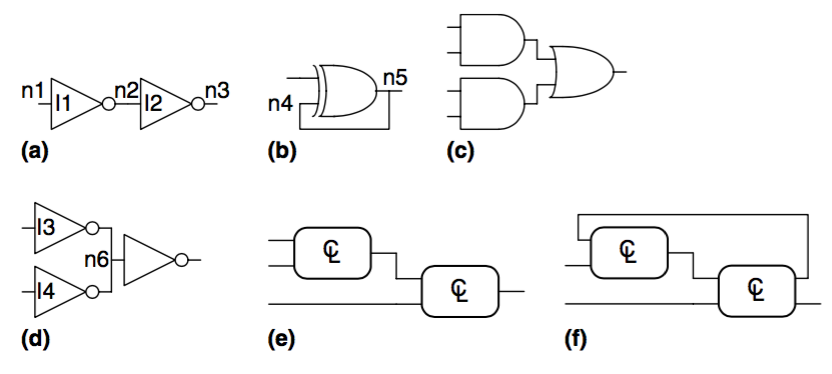
\includegraphics{pictures/combinationalCircuitExample.png}
  (a) is combinational. It is constructed from two combinational circuit elements (inverters $I1$ and $I2$). It has three nodes: $n1$, $n2$, and $n3$. $n1$ is an input to the circuit and to $I1$; $n2$ is an internal node, which is the output of $I1$ and the input to $I2$; $n3$ is the output of the circuit and of $I2$. \\
  (b) is \emph{not} combinational, because there is a cyclic path: the output of the XOR feeds back to one of its input. Hence, a cyclic path starting at $n4$ passes through the XOR to $n5$, which returns to $n4$. \\
  (c) is combinational. \\
  (d) is not combinational, because node $n6$ connects to the output terminals of both $I3$ and $I4$. \\
  (e) is combinational, illustrating two combinational circuits connecting to from a larger combinational circuit. \\
  (f) does not obey the rules of combinational composition because it has a cyclic path through the two elements. Depending on the functions of the elements, it may or may not be a combinational circuit. \\

  The functional specification of a combinational circuit is usually expressed as a truth table or a Boolean equation.

  \section{Boolean Equations}
  Boolean equations deal with variables that are either TRUE or FALSE, so they are perfect for describing digital logic.

  \subsection{Terminology}
  The \emph{complement} of a variable, $A$, is its inverse, $\overline{A}$. \\
  The variables or its complement is called a \emph{literal}.
  For example, $A$, $\overline{A}$, $B$, and $\overline{B}$ are literals. \\
  $A$ is called the \emph{true form} of the variable and $\overline{A}$ the complementary form; ``true form'' does not mean that $A$ is TRUE, but merely that $A$ does not have a line over it. \\

  The AND of one or more literals is called a \emph{product} or an \emph{implicant}. \\
  $\overline{A}B$, $A\overline{B}\overline{C}$, and $B$ are all implicants for a function of three variables. \\
  A \emph{minterm} is a product involving all of the inputs to the function.
  $A\overline{B}\overline{C}$ is a minterm for a function of the three variables $A$, $B$, and $C$, but $\overline{A}B$ is not, because it does not involve $C$. \\

  Similarly, the OR of one or more literals is called a \emph{sum}.
  A \emph{maxterm} is a sum involving all of the inputs to the function. $A + \overline{B} + C$ is a maxterm for a function of the three variables $A$, $B$, and $C$.

  \subsection{Sum-of-Products Form}
  A truth table of $N$ inputs contains $2^{N}$ rows, one for each possible value of the inputs. \\
  Each row in a truth value is associated with a minterm that is TRUE for that row. \\
  A Boolean equation can be written for any truth table by summing each of the minterms for which the output, $Y$, is TRUE.
  This is called the \emph{sum-of-products canonical form} of a function because it is the sum (OR) of products (ANDs forming minterms). \\

  The sum-of-products form provides a Boolean equation for any truth table with any number of variables.
  Unfortunately, it does not necessarily generate the simplest equation.

  \section{Boolean Algebra}
  \subsection{Axioms}
  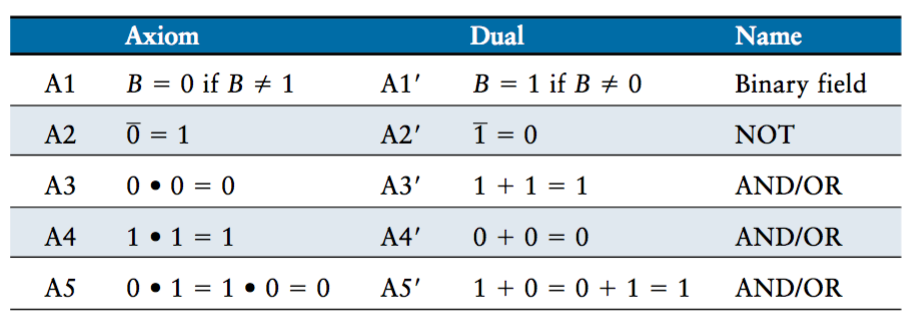
\includegraphics[scale=0.7]{pictures/booleanAlgAxiom.png}

  \subsection{Theorems of One Variable}
  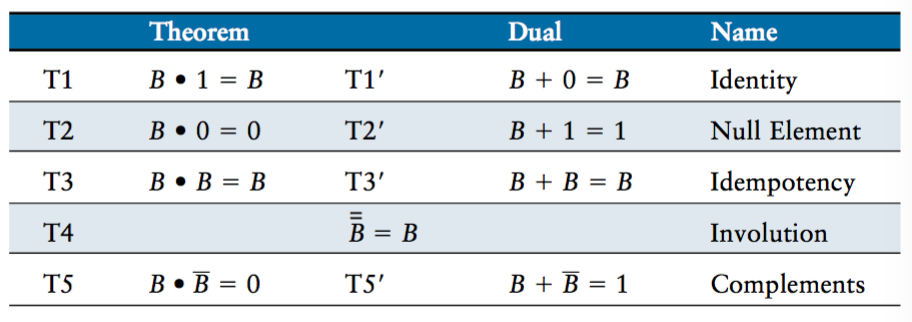
\includegraphics[scale=0.7]{pictures/booleanAlgOneVari.png}

  \subsection{Theorems of Several Variables}
  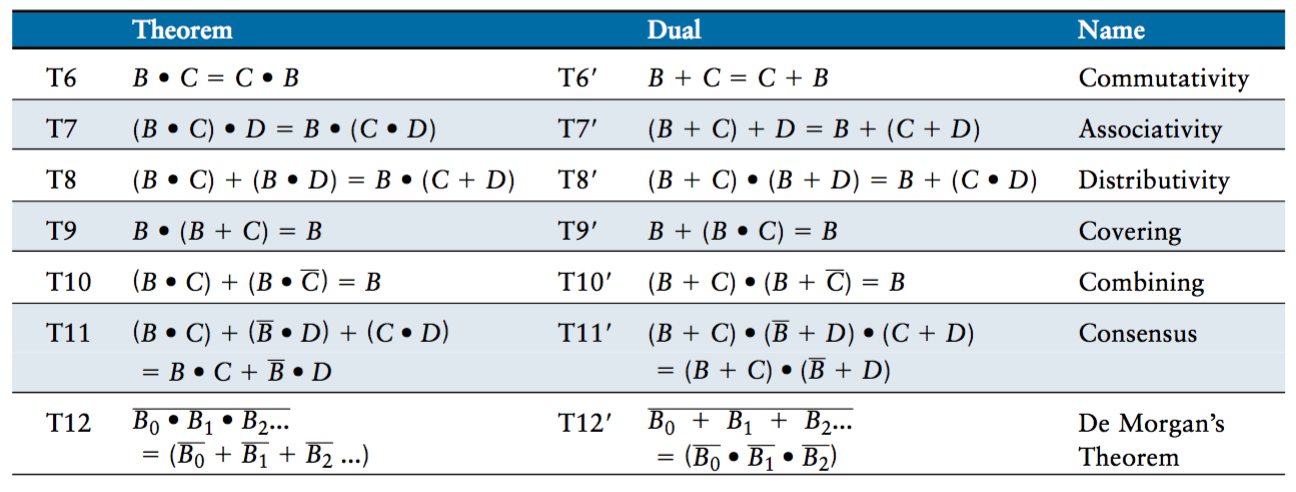
\includegraphics[scale=0.6]{pictures/booleanAlgMultVar.png}

  \section{From Logic to Gates}
  A \emph{schematic} is a diagram of a digital circuit showing the elements and the wires that connect them together. \\

  \textbf{Good Style in Circuit Drawing}:
  \begin{itemize}
    \item Assume all literals (variables and their negations) are available
    \item Rectilinear wires, dots when wires split
    \item Do not draw spaghetti wires for inputs; instead, write each literal as needed
  \end{itemize}

  \section{Multilevel Combinational Logic}
  Logic in sum-of-products form is called \emph{two-level logic} because it consists of literals connected to a level of AND gates connected to a level of OR gates. \\
  Designers often build circuits with more than two levels of logic gates.
  These multilevel combinational circuits may use less hardware than their two-level counterparts. \\
  Bubble pushing is especially helpful in analyzing and designing multilevel circuits.

  \subsection{Hardware Reduction}
  Some logic functions require an enormous amount of hardware when built using two-level logic.
  A notable example is the XOR function of multiple variables. \\
  A three-input XOR can be built out of a cascade of two-input XORs. \\
  Similarly, an eight-input XOR would require 128 eight-input AND gates and one 128-input OR gate for a two level-sum-of-products implementation. A much better option is to use a tree of two-input XOR gates. \\

  ``Best'' has many meanings: fewest gates, fastest, shortest design time, least cost, least power consumption. \\
  ``Best'' circuit in one technology is not necessarily the best in another.
  ANDs and ORs are used often, but in CMOS, NANDs and NORs are more efficient.

  \subsection{Bubble Pushing}
  CMOS circuits prefer NANDs and NORs over ANDs and ORs.
  However, reading the equation by inspection can be difficult. \\
  Bubble pushing is a helpful way to redraw these circuits so that the bubbles cancel out and the function can be more easily determined. \\
  Guidelines for bubble pushing:
  \begin{itemize}
    \item Begin at the output of the circuit and work toward the inputs.
    \item Push any bubbles on the final output back toward the inputs so that you can read an equation in terms of the output.
    \item Working backward, draw each gate in a form so that bubbles cancel. If the current gate has an input bubble, draw the preceding gate with an output bubble. If the current gate does not have an input bubble, draw the preceding gate without an output bubble.
  \end{itemize}

  \section{Combinational Building Blocks}
  Combinational logic is often grouped into larger building blocks to build more complex systems.
  This is an application of the principle of abstraction, hiding the unnecessary gate-level details to emphasize the function of the building block.

  \subsection{Multiplexers}
  \emph{Multiplexers}, also known as \emph{mux}, are among the most commonly used combinational circuits.
  They choose an output from among several possible inputs based on the value of a \emph{select} signal.

  \subsubsection{2:1 Multiplexer}
  \begin{wrapfigure}{r}{0.25\textwidth}
    \centering
    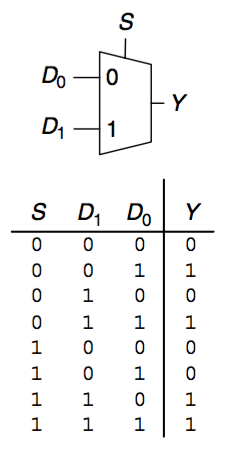
\includegraphics[width=0.25\textwidth]{pictures/2_1_mux.png}
  \end{wrapfigure}
  Image shows the schematic and truth table for a 2:1 multiplexer with two data inputs, $D_0$ and $D_1$, as select input, $S$, and one output, $Y$. \\
  The multiplexer chooses between the two data inputs based on the select:
  if $S = 0$, $Y = D_0$, and if $S = 1$, $Y = D_1$.  \\
  $S$ is also called a control signal because it controls what the multiplexer does. \\

  Multiplexers can be built from tristate buffers. \\
  The tristate enables are arranged such that, at all times, exactly one tristate buffer is active. \\
  When $S = 0$, tristate $T_0$ is enabled, allowing $D_0$ to flow to $Y$. \\
  When $S = 1$, tristate $T_1$ is enabled, allowing $D_1$ to flow to $Y$.

  \subsubsection{Wider Multiplexers}
  A 4:1 multiplexer has four data inputs and one output.
  Two select signals are needed to choose among the four data inputs.
  The 4:1 mux can be built using sum-of-products logic, tristates, or multiple 2:1 mux. \\

  The product terms enabling the tristates can be formed using AND gates and inverters.
  They can also be formed using a decoder. \\

  In general, an $N:1$ multiplexer needs $log_{2} N$ select lines.

  \subsubsection{Multiplexer Logic}
  Multiplexers can be used as \emph{lookup tables} to perform logic functions.
 \\
  In general, a $2^{N}$-input multiplexer can be programmed to perform any N-input logic functions by applying 0's and 1's to the appropriate data inputs. \\
  By changing the data inputs, the multiplexer can be reprogrammed to perform a different function.

  \subsection{Decoder}
  A decoder has $N$ inputs and $2^{N}$ outputs. \\
  It asserts exactly one of its outputs depending on the input combination.
  The outputs are called \emph{one-hot}, because exactly one is ``hot'' (HIGH) at a given time. \\

  Example of 2:4 decoder and its implementation: \\
  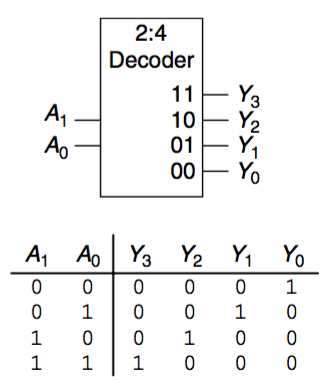
\includegraphics{pictures/2_4_decoder.png}
  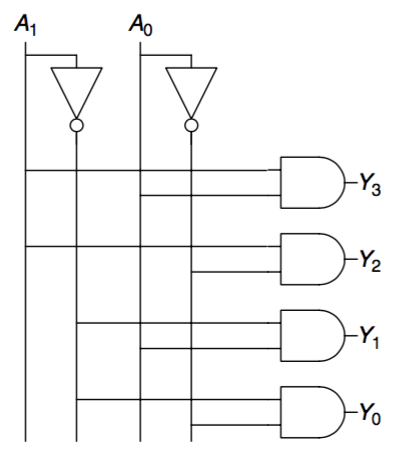
\includegraphics{pictures/2_4_decoder_implementation.png} \\

  \subsubsection{Decoder Logic}
  Decoders can be combined with OR gates to build logic functions. \\
  When using decoders to build logic, it is easiest to express functions as a truth table or in canonical sum-of-products form.
  A $N$-input function with $M$ 1's in the truth table can be built with an $N:2^{N}$ decoder and an $M$-input or gate attached to all of the minterms containing 1's in the truth table.

  \section{Summary So Far}
  A digital circuit is a module with discrete-valued inputs and outputs and a specification describing the function and timing of the module. \\

  The function of a combinational circuit can be given by a truth table or a Boolean equation. The Boolean equation for any truth table can be obtained systematically using sum-of-products or product-of-sums form. \\
  In sum-of-products form, the function is written as the sum (OR) of one or more implicants.
  Implicants are the product (AND) of literals.
  Literals are the true or complementary forms of the input variables.  \\

  Boolean equation can be simplified using the rules of Boolean algebra.
  In particular, they can be simplified into minimal sum-of-products form by combining implicants that differ only in the true and complementary forms of one of the literals: $PA + P\overline{A} = P$. \\

  Logic gates are connected to create combinational circuits that perform the desired function. \\
  Any functions in sum-of-products form can be built using two-level logic with the literals as inputs: NOT gates form the complementary literals, AND gates form the products, and OR gates form the sum. \\
  CMOS circuits favor NAND and NOR gates because these gates can be built directly from CMOS transistors without requiring extra NOT gates. \\
  When using NAND and NOR gates, bubble pushing is helpful to keep track of the inversions. \\

  Logic gates are combined to produce larger circuits such as multiplexers, decoders, and priority circuits. \\
  A multiplexer chooses one of the data inputs based on the select input. \\
  A decoder sets one of the outputs HIGH according to the input. \\
  A priority circuit produces an output indicating the highest priority input. \\

  The timing specification of a combinational circuit consists of the propagation and contamination delays through the circuit. \\
  These indicate the longest and shortest times between an input change and the consequent output change. \\
  Calculating the propagation delay of a circuit involves identifying the critical path through the circuit, then adding up the propagation delays of each element along that path.

  \section{Introduction to Sequential Logic Design}
  The output of sequential logic depend on both current and prior input values. \\
  Hence, sequential logic has memory.
  Sequential logic might explicitly remember certain previous inputs, or it might distill the prior inputs into a smaller amount of information called the \emph {state} of the system. \\
  The state of a digital sequential circuit is a set of bits called \emph{state variables} that contain all the information about the past necessary to explain the future behavior of the circuit.

  \section{Latches and Flip-Flops}
  The fundamental building block of memory is a \emph{bistable} element, an element with two stable states. \\
  An element with $N$ stable states conveys $\log_{2}N$ bits of information, so a bistable element stores one bit. \\
  The state of the cross-coupled inverters is contained in one binary state variable, $Q$.
  The value of $Q$ tells us everything about the past that is necessary to explain the future behavior of the circuit. \\
  Specifically, if $Q = 0$, it will remain 0 forever, and if $Q = 1$, it will remain 1 forever. \\
  The circuit does have another node, $\overline{Q}$, but $\overline{Q}$ does not contain any additional information because if $Q$ is known, $\overline{Q}$ is also known.
  $\overline{Q}$ is also an acceptable choice for the state variable. \\

  When power is first applied to a sequential circuit, the initial state is unknown and usually unpredictable.
  It may differ each time the circuit is turned on. \\

  Although the cross-coupled inverters can store a bit of information, they are not practical because the user has no inputs to control the states. \\
  However, other bistable elements, such as \emph{latches} and \emph{flip-flops}, provide inputs to control the value of the state variable.

  \blfootnote{Just a $Y$ is commonly used for the output of combinational logic, $Q$ is commonly used for the output of sequential logic.}

  \newpage

  \subsection{SR Latch}
  \begin{wrapfigure}{r}{0.25\textwidth}
    \centering
    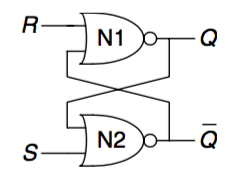
\includegraphics[width=0.25\textwidth]{pictures/srLatch.png}
  \end{wrapfigure}

  \emph{SR latch} is one of the simplest sequential circuit as it is composed of two cross-coupled NOR gates. \\
  The latch has two inputs, $S$ and $R$, and two outputs, $Q$ and $\overline{Q}$. \\
  The SR latch is similar to the cross-coupled inverters, but its state can be controlled through the $S$ and $R$ inputs, which \emph{set} and \emph{reset} the output $Q$. \\

  Consider the four possible combinations of $R$ and $S$:
  \begin{itemize}
    \item[\emph{Case I:}] $R = 1, S = 0$ \\
    N1 sees at least one TRUE input, $R$, so it produces a FALSE output on $Q$. N2 sees both $Q$ and $S$ FALSE, so it produces a TRUE output on $\overline{Q}$.
    \item[\emph{Case II:}] $R = 0, S = 1$ \\
    N1 receives inputs of 0 and $\overline{Q}$. Because we don't yet know $\overline{Q}$, we can't determine the output $Q$. N2 receives at least one TRUE input, $S$, so it produces a FALSE output on $\overline{Q}$. Now we can revisit N1, knowing that both inputs are FALSE, so the output $Q$ is TRUE.
    \item[\emph{Case III:}] $R = 1, S = 1$ \\
    N1 and N2 both set at least one TRUE input ($R$ or $S$), so each produces a FALSE output. Hence $Q$ and $\overline{Q}$ are both FALSE.
    \item[\emph{Case IV:}] $R = 0, S = 0$ \\
    N1 receives inputs of 0 and $\overline{Q}$. Because we don't yet know $\overline{Q}$, we can't determine the output. N2 receives inputs of 0 and $Q$. Because we don't yet know $Q$, we can't determine the output. Now we are stuck. This is reminiscent of the cross-coupled inverters. But we know that $Q$ must either be 0 or 1. So we can solve the problem by checking what happens in each of these sub-cases.
    \item[\emph{Case IVa:}] $Q = 0$ \\
    Because $S$ and $Q$ are FALSE, N2 produces a TRUE output on $\overline{Q}$. Now N1 receives one TRUE input, $\overline{Q}$, so its output, $Q$, is FALSE.
    \item[\emph{Case IVb:}] $Q = 1$ \\
    Because $Q$ is TRUE, N2 produces a FALSE output on $\overline{Q}$. Now N1 receives two FALSE inputs, $R$ and $\overline{Q}$, so its output, $Q$, is TRUE.
  \end{itemize}

  Suppose $Q$ has some known prior value, $Q_{prev}$, before we enter Case IV. $Q_{prev}$ is either 0 or 1, and represents the state of the system.
  When $R$ and $S$ are 0, $Q$ will remember this old value, $Q_{prev}$, and $\overline{Q}$ will be its complement, $\overline{Q}_{prev}$.
  This circuit has memory. \\

  Like the cross-coupled inverters, the SR latch is a bistable element with one bit of state stored in $Q$.
  However, the state can be controlled through the $S$ and $R$ inputs. \\
  When $R$ is asserted, the state is reset to 0. \\
  When $S$ is asserted, the state is set to 1. \\
  When neither is asserted, the state retains its old value.

  \subsection{D Latch}
  The SR latch is awkward because it behaves strangely when both $S$ and $R$ are simultaneously asserted.
  Moreover, the $S$ and $R$ inputs conflate the issues of \emph{what} and \emph{when}.
  Asserting one of the inputs determines not only \emph{what} the state should be but also \emph{when} it should change. \\

  \begin{wrapfigure}{r}{0.8\textwidth}
    \centering
    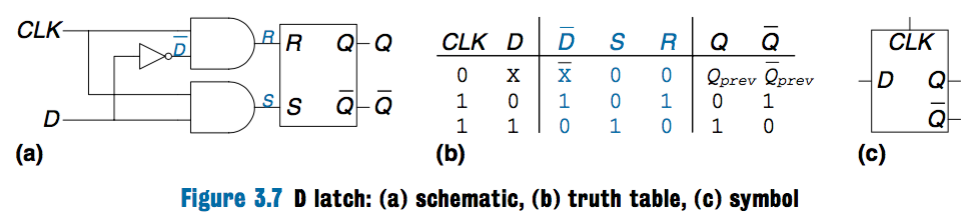
\includegraphics[width=0.8\textwidth]{pictures/dLatch.png}
  \end{wrapfigure}
  The D latch has two inputs.
  The \emph{data} input, $D$, controls what the next state should be.
  The \emph{clock} input, $CLK$, controls when the state should change. \\
  The clock controls when data flows through the latch. \\
  When $CLK = 1$, the latch is \emph{transparent}.
  The data at $D$ flows through to $Q$ as if the latch were just a buffer. \\
  When $CLK = 0$, the latch is \emph{opaque}.
  It blocks the new data from flowing through to $Q$, and $Q$ retains the old value. \\
  The D latch updates its state continuously $CLK = 1$.
  \newpage
  \subsection{D Flip-Flop}
  \begin{wrapfigure}{r}{0.3\textwidth}
    \centering
    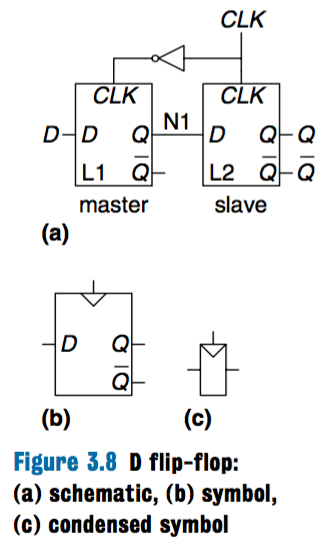
\includegraphics[width=0.3\textwidth]{pictures/dFlipFlop.png}
  \end{wrapfigure}
  A \emph{D flip-flop} can be built from two back-to-back D latches controlled by complementary clocks. \\
  The first latch, $L1$, is called the \emph{master}. \\
  The second latch, $L2$, is called the \emph{slave}. \\
  The node between them is named $N1$. \\
  A symbol for the D flip-flop is given in the figure (b). \\
  When the $\overline{Q}$ output is not needed, the symbol can be condensed as in figure (c). \\

  When $CLK = 0$, the master latch is transparent and the slave is opaque.
  The value at $D$ propagates through to $N1$. \\
  When $CLK = 1$, the master goes opaque and the slave becomes transparent.
  The value at $N1$ propagates through to $Q$, but $N1$ is cut off from $D$.
  Hence, the value at $D$ immediately before the clock rises from 0 too 1 gets copied to $Q$ immediately after the clock rises. \\
  At other times, $Q$ retains its old value, because there is always an opaque latch blocking the path between $D$ and $Q$. \\

  A \emph{D flip-flop} copies $D$ to $Q$ on the rising edge of the clock, and remembers its state at all other times. \\

  A D flip-flop is also known as a \emph{master-slave flip-flop}, an \emph{edge-triggered flip-flop}, or a \emph{positive edge-triggered flip-flop}.

  \subsection{Register}
  A $N$-bit register is a bank of $N$ flip-flops that share a common $CLK$ input, so that all bits of the register are updated at the same time. \\
  Registers are the key building block of most sequential circuits. \\

  For a 32-bit architectures, a register would typically have 32 flip-flops in parallel (i.e. one for each bit). \\
  A \emph{register file} is a way of organizing registers. \\
  \includePicture{1.0}{pictures/registerFile.png}{A register file.} \label{registerFile}

  \subsubsection{Reading from a Register File}
  The values of all 32 registers go through two multiplexers. \\
  The first multiplexer determines which register value will be routed to the 1\textsuperscript{st} output. \\
  The second multiplexer determines which register value will be routed to the 2\textsuperscript{nd} output. \\
  It will take 5 select lines to uniquely identify each source register (when there are 32 registers).

  \subsubsection{Writing to a Register File}
  The address of the register $d$, is routed through a decoder which determines which D flip-flop to write to. \\
  When the $d^{\text{th}}$ decoder line and the \emph{RegWrite} line are both 1, they pass a 1 through the $d^{\text{th}}$ AND gate and raise the $C$ input of the $d^{\text{th}}$ D flip-flop to 1. \\
  The data will now be written to Register $\$d^{\text{th}}$.

  \section{Finite State Machines}
  Synchronous sequential circuits can be drawn in the forms called \emph{finite state machines (FSMs)}.
  The name comes from a circuit with $k$ registers can be in one of a finite number ($2^{k}$) of unique states. \\
  A FSM has $M$ inputs, $N$ outputs, and $k$ bits of state.
  It also receives a clock and, optionally, a reset signal. \\
  An FSM consists of two blocks of combinational logic, \emph{next state logic} and \emph{output logic}, and a register that stores the state.
  On each clock edge, the FSM advances to the next state, which was computed based on the current state and inputs. \\
  Finite state machines provides a systematic way to design synchronous sequential circuits given a functional specification.

  Two general classes of finite state machines, characterized by their functional specifications. \\
  In \emph{Moore machines}, the outputs depend only on the current state of the machine. \\
  In \emph{Mealy machines}, the outputs depend on both the current state and the current inputs. \\

  \subsection{State Transition Diagram}
  \begin{wrapfigure}{r}{0.4\textwidth}
    \centering
    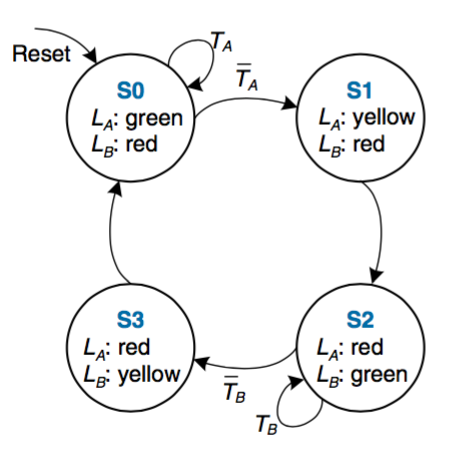
\includegraphics[width=0.4\textwidth]{pictures/stateTransistionDiagram.png}
  \end{wrapfigure}
  A \emph{state transition diagram} indicates all the possible states of the system and the transitions between these states. \\
  In a state transition diagram, circles represent states and arcs represent transitions betweens states. \\
  The transitions take place on the rising edge of the clock; the clock can hidden on the diagram because it is always present in a synchronous sequential circuit.
  In addition, the clock only controls when the transitions should occur, whereas the diagram indicates which transitions occur. \\
  If a state has multiple arcs leaving it, the arcs are labeled to show what input triggers each transition.
  In the image, when in state $S0$, the system will remain in that state if $T_{A}$ is TRUE and move to $S1$ if $T_{A}$ is FALSE. \\
  If a state has a single arc leaving it, that transition always occurs regardless of the inputs.
  In the image, when in state $S1$, the system will always move to $S2$. \\

  \subsection{State Transition Table}
  \includePicture{0.8}{pictures/stateTTableStateEncode.png}{Example Transition Table and its Encoding}
  A \emph{state transition table} indicates for each state and input, what the next state, $S'$, should be.
  If the next state does not depend on a particular input, the don't care symbol (X) is used. \\
  To build a real circuit, the states and outputs must be assigned \emph{binary encodings}.

  \subsection{State Encoding}
  If the state and output encodings were selected arbitrarily, a different choice would have resulted in a different circuit. \\
  Then how to determine the encoding that produces the circuit with the fewest logic gates or the shortest propagation delay?
  There is not simply method to find the best encoding. \\
  It is possible to choose a good encoding by inspection, so that related states share bits. \\

  An important decision in state encoding is the choice between binary encoding and one-hot encoding. \\
  With \emph{binary encoding}, each state is represented as a binary number.
  Because $K$ binary numbers can be represented by $\log_{2}K$ bits, a system with $K$ states only needs $\log_{2}K$ bits of state. \\

  In \emph{one-hot encoding},  a separate bit of state is used for each state.
  It is called one-hot because only one bit is ``hot'' or TRUE at any time.
  \begin{ex}
    A one-hot encoded FSM with three states would have state encodings of 001, 010, and 100.
  \end{ex}
  Each bit of state is stored in a flip-flop, so one-hot encoding requires more flip-flops than binary encoding.
  However, with one-hot encoding, the next-state and output logic is often simpler, so fewer gates are required. \\

  Another encoding is the \emph{one-cold} encoding, in which $K$ states are represented with $K$ bits, exactly one of which is FALSE.

  \subsection{FSM Review} \label{FSM_Review}
  Finite state machines are a powerful way to systematically design sequential circuits from a written specification. \\
  Procedure to design an FSM:
  \begin{enumerate}
    \item[>] Identify the inputs and outputs.
    \item[>] Sketch a state transition diagram.
    \item[>] For a Moore machine:
    \begin{enumerate}
      \item[-] Write a state transition table.
      \item[-] Write an output table.
    \end{enumerate}
    \item[>] For a Mealy machine:
    \begin{enumerate}
      \item[-] Write a combined state transition and output table.
    \end{enumerate}
    \item[>] Select state encodings---selection affects the hardware design.
    \item[>] Write Boolean equations for the next state and output logic.
    \item[>] Sketch the circuit schematics.
  \end{enumerate}

  \section{Summary So Far}
  In contrast to combinational logic, whose outputs depend solely on the current inputs, sequential logic outputs depend on both current and prior inputs.
  Sequential logic remembers information about prior inputs.
  This memory is called the state of the logic. \\

  Sequential circuits can be difficult to analyze and are easy to design incorrectly.
  An important element is the flip-flop, which receives a clock and an input, $D$, and produces an output, $Q$.
  The flip-flop copies $D$ to $Q$ on the rising edge of the clock and otherwise remembers the old state of $Q$.
  A group of flip-flops sharing a common clock is called a register.
  Flip-flops may also receive reset or enable control signals. \\

  Finite state machines are a powerful technique for designing sequential circuits.
  For procedure on designing an FSM, refer to \ref{FSM_Review} (FSM Review). \\

  Synchronous sequential circuits have a timing specification including to clock-to-$Q$ propagation and contamination delay, $t_{pcq}$ and $t_{ccq}$, and the setup and hold times, $t_{setup}$ and $t_{hold}$. \\
  For correct operation, their inputs must be stable during an aperture time that starts a setup time before the rising edge of the clock and ends a hold time after the rising edge of the clock. \\

  The minimum cycle time, $T_{c}$, of the system is equal to the propagation delay, $t_{pd}$, through combinational logic plus $t_{pcq} + t_{setup}$ of the register. \\
  For correct operation, the contamination delay through the register and combinational logic must be greater than $t_{hold}$.
  Hold time does not affect the cycle time. \\

  Overall performance is measured in latency and throughput.
  The latency is the time required for a token to pass from start to end.
  The throughput is the number of tokens that the system can process per unit time.
  Parallelism improves the system throughput.

  \section{Memory Technologies}
  There are four primary technologies used in memory hierarchies. \\
  Main memory is implemented from DRAM (dynamic random access memory), while levels closer the processor (caches) uses SRAM (static random access memory). \\
  DRAM is less costly per bit than SRAM, although it is substantially slower.
  The price difference arises because DRAM uses significantly less area per bit of memory, and DRAMs thus have larger capacity for the same amount of silicon. \\

  \subsection{SRAM Technology}
  SRAMs are simply integrated circuits that are memory arrays with (usually) a single access port that can provide either a read or a write. \\
  SRAMs have a fixed access time to any datum, though read and write access times may differ. \\
  SRAMs don't need to refresh and so the access time is very close to the cycle time. \\
  SRAMs typically use six to eight transistors per bit to prevent the information from being disturbed when read. \\
  SRAM needs only minimal power to retain the charge in standby mode.

  \subsection{DRAM Technology}
  In a SRAM, as long as power is applied, the value can be kept indefinitely. \\
  In a dynamic RAM, the value kept in a cell is stored as a charge in a capacitor.
  A single transistor is then used to access this stored charge, either to read the value or to overwrite the charge stored there. \\
  Because DRAMs use only a single transistors per bit of storage, they are much denser and cheaper per bit than SRAM. \\
  As DRAMs store the charge on a capacitor, it cannot be kept indefinitely and must periodically be refreshed.
  Hence this memory structure is dynamic, as opposed to the static storage in an SRAM cell. \\

  To refresh the cell, we merely read its contents and write it back.
  The charge can be kept for several ms.
  If every bit had to be read out of the DRAM and then written back individually, the DRAM would be constantly refreshed, leaving no time to access it. \\
  DRAMs use a two-level decoding structure, which allows the ability to refresh an entire \emph{row} (which shares a word line) with a read cycle followed immediately by a write cycle. \\

  The row organization that helps with refresh also helps with performance.
  To improve performance, DRAMs buffer rows for repeated access.
  The buffer acts like a SRAM; by changing the address, random bits can be accessed in the buffer until the next row access.
  This capability improves the access time significantly, since the access time to bits in the row is much lower.
  When the row is in the buffer, it can be transferred by successive addresses at whatever the width of the DRAM is, or by specifying a block transfer and the starting address within the buffer. \\

  To further improve the interface to processors, DRAMs added clocks which is called Synchronous DRAMs or SDRAMs.
  The advantage is that the use of a clock eliminates the time for the memory and processor to synchronize.
  The speed advantage of synchronous DRAMs come from the ability to transfer the bits in the burst without having to specify additional address bits.
  Instead, the clock transfer the successive bits in a burst. \\
  \emph{Double Data Rate} (DDR) SDRAM is the fastest currently available.
  Data transfer on both the rising and falling edge of the clock, thereby getting twice as much bandwidth based on the clock rate and the data width. \\

  Sustaining the bandwidth requires clever organization \emph{inside} the DRAM.
  The DRAM can be internally organized, instead of just a faster row buffer, to read or write from multiple \emph{banks}, which each having its own row buffer.
  Sending an address to several banks permits them all to read or write simultaneously.
  The rotating access scheme is called \emph{address interleaving}.

  \section{Multiplication}
  \includePicture{0.9}{pictures/multiplication.png}{Multiplication Hardware Version 1.0}
  The first operand is called the \emph{multiplicand} and the second the \emph{multiplier}.
  The final result is called the \emph{product}. \\\
  Number of bits in the product is considerably larger than the number in either the multiplicand or the multiplier.
  If ignoring the sign bit, the length of the multiplication of an $n$-bit multiplicand and an $m$-bit multiplier is a product that is $n + m$ bits long.
  So $n + m$ bits are required to represent all possible products.

  \section{Floating Point}
  A number in scientific notation that has no leading 0s is called a \emph{normalized} number, which is the usual way to write it. \\
  \emph{Floating point} is computer arithmetic that represents numbers in which the binary point is not fixed. \\
  A standard scientific notation for reals in normalized form offers tree advantages:
  \begin{enumerate}
    \item It simplifies exchange of data that includes floating-point numbers.
    \item It simplifies the floating-point arithmetic algorithms to know that numbers will always be in this form.
    \item It increases the accuracy of the numbers that can be stored in a word, since the unnecessary leading 0s are replaced by real digits to the right of the binary point.
  \end{enumerate}

  \subsection{Floating-Point Representation}
  \includePicture{0.8}{pictures/mipsFloat.png}{Representation of a MIPS \emph{single precision} floating-point number.}
  $s$ is the sign of the floating-point number (1 meaning negative).
  \emph{exponent} is the value of the 8-bit exponent field (including the sign of the exponent).
  \emph{fraction} is the 23-bit number. \\
  Generally, floating-point numbers are of the form: $$(-1)^{s} \times F \times 2^{E}$$
  F involves the value in the fraction field and E involves the value in the exponent field.

  \blfootnote{\emph{overflow}: positive exponent becomes too large to fit in the exponent field}
  \blfootnote{\emph{underflow}: negative exponent becomes too large to fit in the exponent field}

  A \emph{double precision} floating-point number is represented in two 32-bit words.
  The exponent is the value of the 11-bit exponent field.
  Fraction is the 52-bit number in the fraction field. \\
  \includePicture{0.85}{pictures/floatingPoints.png}{IEEE 754 encoding of floating-point numbers.}

  This is also known as the \emph{IEEE 754 floating-point standard}.
  This standard has greatly improved both the ease of porting floating-point programs and the quality of computer arithmetic. \\
  In IEEE 754, the leading 1-bit of normalized binary number is implicit, so the number is actually 24 bits long in single precision. \\

  For the fractional part, suppose we number the bits of the fraction from left to right $s1$, $s2$, $s3$, \dots, then the value is
  $$(-1)^{S} \times (1 + (s1 \times 2^{-1}) + (s2 \times 2^{-2}) + (s3 \times 2^{-3}) + (s4 \times 2^{-4}) + \dots) \times 2^{E}$$

  IEEE 754 uses a bias of 127 for single precision exponent. \\
  The exponent bias for double precision is 1023. \\
  So the value represented by a floating-point number is really
  $$(-1)^{S} \times (1 + \text{Fraction}) \times 2^{(\text{Exponent} - \text{Bias})}$$

  \subsection{Floating-Point Addition}
  \begin{itemize}
    \item[1.] Compare the exponents of the two numbers; shift the smaller number to the right until its exponent would match the larger exponent.
    \item[2.] Add the significants.
    \item[3.] Normalize the sum, either shifting right and incrementing the exponent or shifting left and decrementing the exponent.
    \item[>] Overflow or underflow? If yes, Exception. Otherwise, continue.
    \item[4.] Round the significant to the appropriate number of bits.
    \item[>] Still normalized? If no, then step 3. Otherwise, done.
  \end{itemize}
  \includePicture{0.7}{pictures/floatingAddition.png}{Arithmetic unit for floating-point addition.}

  \subsection{Floating-Point Multiplication}
  \begin{itemize}
    \item[1.] Add the biased exponents of the two numbers, subtracting the bias from the sum to get the new biased exponent.
    \item[2.] Multiply the significants.
    \item[3.] Normalize the product if necessary, shifting it right and incrementing the exponent.
    \item[>] Overflow or underflow? If yes, Exception. Otherwise, continue.
    \item[4.] Round the significant to the appropriate number of bits.
    \item[>] Still normalized? If no, then Step 3. Otherwise, continue.
    \item[5.] Set the sign of the product to positive if the signs of the original operands are the same; if they differ, make the sign negative.
  \end{itemize}

  \section{Introduction to the Processor}
  A subset of the core MIPS instruction set will be examined:
  \begin{enumerate} \label{instruction_classes}
    \item[>] The memory-reference instructions \emph{load word} (lw) and \emph{store word} (sw)
    \item[>] The arithmetic-logical instructions add, sub, AND, OR, and slt
    \item[>] The branch instructions \emph{branch equal} (beq) and \emph{jump} (j)
  \end{enumerate}
  To implement those instructions, the first two steps are identical:
  \begin{enumerate}
    \item Send the \emph{program counter} (PC) to the memory that contains the code and fetch the instruction from that memory.
    \item Read one or two registers, using fields of the instruction to select the registers to read. For the load word instruction, only need to read one register, but most other instructions require reading two registers.
  \end{enumerate}
  After the two steps, the required actions depend on the instruction class.
  For each of the three instructions classes (\ref{instruction_classes}), the actions are largely the same, independent of the exact instruction. \\
  The simplicity and regularity of the MIPS instruction set simplifies the implementation by making the execution of many of the instruction classes similar. \\

  All instruction classes, except jump, use the arithmetic-logical unit (ALU) after reading the registers.
  The memory-reference instructions use the ALU for an address calculation, the arithmetic-logical instructions for the operation execution, and branches for comparison. \\
  After using the ALU, the actions required to complete various instruction classes differ. \\
  A memory-reference instruction will need to access the memory either to read data for a load or write data for a store. \\
  An arithmetic-logical or load instruction must write the data from the ALU or memory back into a register. \\
  For a branch instruction, it may be required to change the next instruction address based on the comparison; otherwise, the PC should be incremented by 4 to get the address of the next instruction.

  \section{Building a Data-path}
  \includePicture{0.7}{pictures/readingFetchingInstruction.png}{A portion of the data-path used for fetching instructions and incrementing the program counter.}
  A \emph{data-path element} is a unit used to operate within a processor.
  In the MIPS implementation, the data-path element include the instruction and data memories, the register file, the ALU, and adders. \\
  To execute any instruction, start by fetching the instruction from memory.
  Then increment the program counter so that it points at the next instruction, 4 bytes later. \\
  Refer to the figure above for how the elements are combined, forming a data-path that fetches instructions and increments the PC. \\

  A \emph{R-type \emph{or} R-format} is an arithmetical-logical instruction since they perform. \\
  All R-format instructions read two registers, perform an ALU operation on the contents of the register, and write the result to a register. \\

  Through a register file, it contains the register state of the computer and the ALU needs to operate on the values read from the registers. \\
  R-format instructions have three register operands, to read two data words from the register file and write one data word into the register file for each instruction. \\
  For each data word to be read from the register, an input to the register file is needed that will carry the value that has been read from the registers. \\
  To write a data word, two inputs are needed: one to specify the register number to be written and one to supply the \emph{data} to be written into the register. \\
  The register file always outputs the contents of whatever register numbers are on the Read register inputs.
  However, writes are controlled by the write control signal, which must be asserted for a write to occur at the clock edge. \\

  Thus, we need a total of four inputs (three for register number and one for data) and two outputs (both for data).
  The register number inputs are 5 bits wide to specify one of 32 registers ($32 = 2^{5}$), whereas the data input and two data output buses are each 32 bits wide (each word is 32 bits).

  \subsection{R-Format ALU Operations}
  Two elements are needed to implement R-format ALU operations: register file (\ref{registerFile}) and the ALU. \\

  The register file contains all the registers and has two read ports and one write port.
  The register file outputs the contents of the registers corresponding to the Read register inputs on the outputs; no other control inputs are needed. \\
  Note that a register write must be explicitly indicated by asserting the write control signal, $RegWrite$.
  Writes are edge-triggered, so that all write inputs must be valid at the clock edge. \\

  The inputs carrying the register number to the register file are all 5 bites wide, whereas the lines carrying data values are 32 bits wide. \\
  The operation to be performed by the ALU is controlled with the ALU operation signal, which will be 4 bits wide.

  \subsection{Memory-Reference Operations}
  Consider $lw$ and $sw$ instructions.
  They compute a memory address by adding the base register to the 16-bit signed offset field contained in the instruction. \\
  If the instruction is a store, the value to be stored must also be read from the register file where it resides in the destination register. \\
  If the instruction is a load, the value read from memory must be written into the register file in the specified register. \\
  Thus, both register and the ALU are required in addition to more. \\

  \includePicture{0.75}{pictures/elementsFormemoryReference.png}{Two units needed for loads and stores. In addition to the register file and ALU.}

  We need a unit to \emph{sign-extend} the 16-bit offset field in the instruction to a 32-bit signed value, and a data memory unit to read from or write to.
  A \emph{sign-extend} is to increase the size of a data item by replicating the high-order sign bit of the original data item in the high-order bits of the larger, destination data item. \\
  The data memory must be written on store instructions; hence, data memory has read and write control signals, an address input, and an input for the data to be written into memory. \\
  Refer to figure above for the two units required.

  \subsection{Branch Operations}

\end{document}
